    
\chapter{Kana II}

\begin{center}
\begin{Large}
第4課: Kana II: Katakana カタカナ  
\end{Large}
\end{center}
 
\par{ In the previous lesson, we learned about how Japanese is a mixed script of four systems in one. Of these four systems, two of them are \emph{Kana }systems: \emph{Hiragana }and \emph{Katakana }. The previous lesson was all about learning the individual symbols of \emph{Hiragana }. In this lesson, our goal will be to learn all the individual symbols for \emph{Katakana }. }

\par{ \emph{Hiragana }and \emph{Katakana }both represent the same sound combinations (morae). As such, there won't be any differences in pronunciation between an \slash a\slash  written in \emph{Hiragana }and one written in \emph{Hiragana }. However, the two scripts are used in different circumstances. Their rules for other aspects of spelling such as long vowel notation are also not exactly the same. For now, we will focus solely on learning the individual symbols of \emph{Katakana }. As you will soon see, there are more symbols to learn in \emph{Katakana }than there is for \emph{Hiragana }. This means you have plenty of work ahead of you in this lesson. }
      
\section{Katakana カタカナ}
 
\par{ Of the two \emph{Kana }systems, \emph{Katakana }is the least used. However, that doesn't mean it isn't used, and it doesn't mean that it isn't important to learn. One cannot properly read Japanese without knowing both systems. The two systems are still used in different ways. The way they're used also affects how complex the systems are. \emph{Katakana }, as you will see, has an additional set of combinations not used in \emph{Hiragana }. This means it'll take a little more effort to memorize \emph{Katakana }than \emph{Hiragana }. With that being said, let's begin.  }

\begin{center}
\emph{KATAKANA }
\end{center}

\par{ The basic symbols of \emph{Katakana }, just as was the case with \emph{Hiragana }, are organized into a chart called the \emph{Gojūonzu }. This chart is shown below with each basic symbol. Just like for \emph{Hiragana }, notice how the stoke orders are listed and how all the allophones of sounds we've learned about are shown in their respective columns. }
 
\begin{figure}[h]
\centering

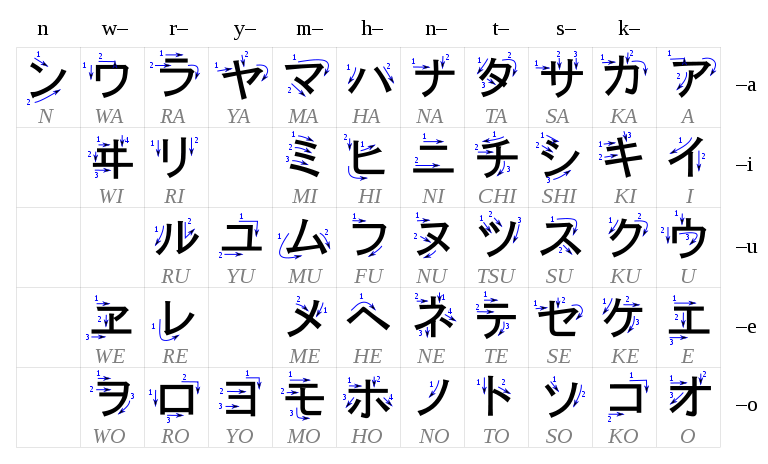
\includegraphics[width=0.9\textwidth]{figs/第01章/第4課:_katakana_fig/768px_Table_katakana.svg.png}

\end{figure}

\par{\textbf{Curriculum Note }: Print this sheet out and have it on hand as we continue moving forward. It will be u seful while you memorize both \emph{Kana }systems. Once we learn about Chinese characters ( \emph{Kanji }), we'll learn how they're all three used along with English letters to write Japanese. }

\par{\textbf{Usage Notes: }}

\par{  Of these characters, all of them except the symbols for \emph{we }and \emph{wi }\emph{ }are typically used. These two characters live on only in names, place names, and old literature. Because there is the chance you will encounter them, when you do see them, read them as "e" and "i" respectively as the "w" has dropped from their actual pronunciations. This is largely why the symbols are no longer seen today. }

\par{ Similarly, the symbol for \emph{wo }is usually pronounced by "o" by most speakers. However, the traditional pronunciation "wo" is still heard depending on personal preference, dialect, as well as occasion. For instance, in music, singers tend to be conservative in pronunciation. This is also the case when people slow down their speech to purposefully enunciate every sound clearly. Unlike in \emph{Hiragana }, th e \emph{Katakana }symbol for \emph{wo }is hardly used at all. This means you won't get many opportunitie s to see it actually used. }

\par{ Of these characters, all but the symbols for \emph{we }, \emph{wi }, \emph{wo }, and \emph{n }can start words. The symbols for \emph{we }and \emph{wi }are deemed obsolete. Also, the symbol for \emph{wo }is only used in names or as a grammatical word that cannot stand alone, which we will learn about later. }

\par{\textbf{Handwriting Notes }: }

\par{1. Write strokes from top to bottom and left to right. \hfill\break
2. Horizontal strokes come before vertical strokes. \hfill\break
3. Take especial note to the stroke orders of シ and ツ.  For シ, its third stroke is irregularly written from the bottom upward, which is how you can distinguish it from ツ, which is written regularly. \hfill\break
4. Also take note of the stroke orders of ソ and ン. For ン, its second stroke is irregularly written from the bottom upward, which is how you can distinguish it from ソ, which is written regularly. \hfill\break
5. When there are horizontal strokes that span the length of the symbol, those strokes aren't first from top to bottom regardless if other strokes may start higher up. Take キ as an example. }

\begin{center}
\textbf{Examples } 
\end{center}

\par{ As your first chance at reading practice, below are 60 common words that are spelled in \emph{Katakana }. Although it's not necessary that you memorize them all now, you'll find that many of them are words you're already very familiar with. }

\begin{ltabulary}{|P|P|P|P|P|P|}
\hline 

Access &  \textbf{ア }クセス & Assistant & ア \textbf{シ }スタント & ASEAN & ア \textbf{セ }アン \\ \cline{1-6}

Africa & ア \textbf{フリカ }& America & ア \textbf{メリカ }& Aluminum & ア \textbf{ルミ }\\ \cline{1-6}

Good-looking guy & イ \textbf{ケメン }& Italy & イ \textbf{タリア }& Earbud & イ \textbf{ヤ }ホン \\ \cline{1-6}

Air conditioning & エ \textbf{アコン }& Eroticism &  \textbf{エ }ロ & Oceania & オ \textbf{セアニア }\\ \cline{1-6}

Offline & オ \textbf{フラ }イン & Cocktail &  \textbf{カ }クテル & Custom &  \textbf{カ }スタム \\ \cline{1-6}

Sponge cake & カ \textbf{ステラ }& Camera &  \textbf{カ }メラ & Karaoke & カ \textbf{ラオケ }\\ \cline{1-6}

Calcium & カ \textbf{ルシ }ウム & Mouse &  \textbf{マ }ウス & Christ & キ \textbf{リスト }\\ \cline{1-6}

Classmate & ク \textbf{ラスメ }イト & Christmas & ク \textbf{リス }マス & Koala &  \textbf{コ }アラ \\ \cline{1-6}

Coin &  \textbf{コ }イン & Siren &  \textbf{サ }イレン & Santa &  \textbf{サ }ンタ \\ \cline{1-6}

System &  \textbf{シ }ステム & Scenario & シ \textbf{ナリオ }& Restaurant &  \textbf{レ }ストラン \\ \cline{1-6}

Hormone & ホルモン & Synchronize & シ \textbf{ンクロ }& Stress & ス \textbf{ト }レス \\ \cline{1-6}

Centi(meter) &  \textbf{セ }ンチ & Seoul &  \textbf{ソ }ウル & Solo &  \textbf{ソ }ロ \\ \cline{1-6}

Towel &  \textbf{タ }オル & Tennis &  \textbf{テ }ニス & Toilet &  \textbf{ト }イレ \\ \cline{1-6}

Hotel &  \textbf{ホ }テル & Minus & マ \textbf{イナス }& Nylon &  \textbf{ナ }イロン \\ \cline{1-6}

Tomato &  \textbf{ト }マト & Ton &  \textbf{ト }ン & Knife &  \textbf{ナ }イフ \\ \cline{1-6}

Necktie &  \textbf{ネ }クタイ & Quota &  \textbf{ノ }ルマ & Handkerchief & ハ \textbf{ンカチ }\\ \cline{1-6}

Stapler &  \textbf{ホ }チキス & Marathon & マ \textbf{ラソン }& Milk &  \textbf{ミ }ルク \\ \cline{1-6}

Mexico & メ \textbf{キシコ }& Moscow & モ \textbf{スクワ }& UNESCO & ユ \textbf{ネ }スコ \\ \cline{1-6}

Toyota &  \textbf{ト }ヨタ & Link &  \textbf{リ }ンク & Lemon &  \textbf{レ }モン \\ \cline{1-6}

Russia &  \textbf{ロ }シア & Request & リ \textbf{クエ }スト & Wine &  \textbf{ワ }イン \\ \cline{1-6}

\end{ltabulary}

\begin{center}
\textbf{Diacritics: ゛ \& ゜ }
\end{center}

\par{ The diacritics we learned about last lesson are used in exactly the same way in \emph{Katakana }. These diacritics, the These diacritics are the ゛ ( \emph{da \textbf{kuten }\slash ni \textbf{gori }}↓) and the ゜ ( \emph{ha \textbf{ndakuten }}), represent voiced consonants and the consonant \slash p\slash  respectively. }
 
\begin{figure}[h]
\centering

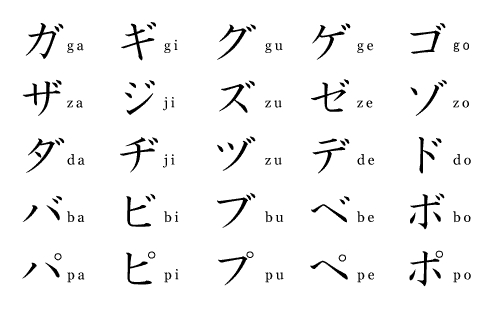
\includegraphics[width=0.9\textwidth]{figs/第01章/第4課:_katakana_fig/Katakana_dakuten_chart.png}

\end{figure}

\par{ Just as was the case with \emph{Hiragana }, you write the basic symbol before adding the diacritics. Additionally, there are two characters for \slash ji\slash  and \slash zu\slash . However, their pronunciations\slash usage aren't 100\% the same. For now, focus on memorizing these symbols. }

\begin{center}
Examples 
\end{center}

\par{ Below are 60 common words that utilize these diacritics. Although it is not necessary that you memorize them all, they are all common words that bring purpose to using \emph{Katakana }as the majority of these words are solely written in \emph{Katakana }. }

\begin{ltabulary}{|P|P|P|P|P|P|}
\hline 

Advice &  \textbf{ア }ドバイス & Radio &  \textbf{ラ }ジオ & England & イ \textbf{ギリス }\\ \cline{1-6}

Pokemon & ポ \textbf{ケモン }& Event & イ \textbf{ベント }& India &  \textbf{イ }ンド \\ \cline{1-6}

Ego &  \textbf{エ }ゴ & Egypt & エ \textbf{ジプト }& Apron &  \textbf{エ }プロン \\ \cline{1-6}

Holland & オ \textbf{ランダ }& Casino &  \textbf{カ }ジノ & Gas &  \textbf{ガ }ス \\ \cline{1-6}

Capsule &  \textbf{カ }プセル & Gift &  \textbf{ギ }フト & Jellyfish & ク \textbf{ラゲ }\\ \cline{1-6}

Mongolia &  \textbf{モ }ンゴル & Golf &  \textbf{ゴ }ルフ & Convenience store & コ \textbf{ンビニ }\\ \cline{1-6}

Size &  \textbf{サ }イズ & Sandals & サ \textbf{ンダル }& Running & ラ \textbf{ンニング }\\ \cline{1-6}

Swimming & ス \textbf{イ }ミング & Pants &  \textbf{ズ }ボン & Celebrity &  \textbf{セ }レブ \\ \cline{1-6}

Zombie &  \textbf{ゾ }ンビ & Diamond & ダ \textbf{イヤモ }ンド & Taipei & タ \textbf{イペイ }\\ \cline{1-6}

Dance &  \textbf{ダ }ンス & Design & デ \textbf{ザ }イン & Digital camera & デ \textbf{ジカメ }\\ \cline{1-6}

TV &  \textbf{テ }レビ & Germany &  \textbf{ド }イツ & Door &  \textbf{ド }ア \\ \cline{1-6}

Dollar &  \textbf{ド }ル & Napkin &  \textbf{ナ }プキン & Trash & ゴ \textbf{ミ }↓ \\ \cline{1-6}

Knob &  \textbf{ノ }ブ & Hiking &  \textbf{ハ }イキング & Basketball &  \textbf{バ }スケ \\ \cline{1-6}

PC & パ \textbf{ソコン }& Bus &  \textbf{バ }ス & Pachinko & パ \textbf{チンコ }\\ \cline{1-6}

Bread &  \textbf{パ }ン & Banana &  \textbf{バ }ナナ & Panda &  \textbf{パ }ンダ \\ \cline{1-6}

Piano & ピ \textbf{アノ }& Visa &  \textbf{ビ }ザ & Pizza &  \textbf{ピ }ザ \\ \cline{1-6}

Vitamin & ビ \textbf{タ }ミン & Video &  \textbf{ビ }デオ & Building &  \textbf{ビ }ル \\ \cline{1-6}

Pink &  \textbf{ピ }ンク & Judea &  \textbf{ユ }ダヤ & Frying pan & フ \textbf{ライパン }\\ \cline{1-6}

Browser & ブ \textbf{ラウザ }& Blog & ブ \textbf{ログ }& Veranda & ベ \textbf{ランダ }\\ \cline{1-6}

McDonald's & マ \textbf{クドナ }ルド & Medal & メ \textbf{ダル }& Memo &  \textbf{メ }モ \\ \cline{1-6}

\end{ltabulary}
\hfill\break

\begin{center}
\textbf{Palatal Sounds }
\end{center}

\par{ Remember that palatal sounds are created by placing the tongue on the hard palate of the mouth. Consonants are naturally palatalized in Japanese when followed by \slash i\slash  or \slash y\slash . For those created with \slash y\slash , shrunken y-sound symbols must be paired with a full-sized i-sound symbol. In \emph{Katakana }, these combinations are as follows. }
 
\begin{figure}[h]
\centering

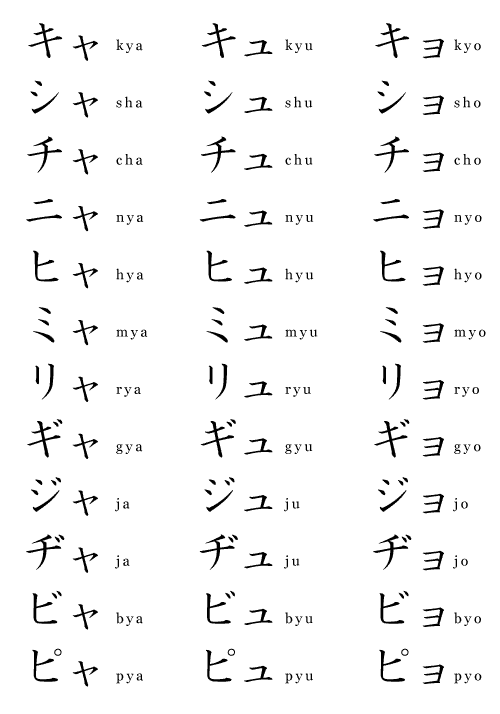
\includegraphics[width=0.9\textwidth]{figs/第01章/第4課:_katakana_fig/Katakana_yuoun_chart.png}

\end{figure}

\par{ Just as was the case with above with there are being two ways to write the says, \slash ji\slash  and \slash zu\slash , the same can be said for \slash ja\slash , \slash ju\slash , and \slash jo\slash . The variants that use ヂ are essentially obsolete as far as spelling actual, common words is concerned. }

\begin{center}
Examples  
\end{center}

\par{ Not all these characters are used as frequently as others. Although some are extremely common, some are only found in certain kinds of words. Others are hard to find without being used with long vowels and consonants. Since we haven't learned what those rules are for the two \emph{Kana }systems, the 30 examples words are limited to words with short consonants and vowels that are actually common expressions. }

\begin{ltabulary}{|P|P|P|P|P|P|}
\hline 

Casual &  \textbf{カ }ジュアル & Curriculum &  \textbf{カ }リキュラム & Cabbage &  \textbf{キャ }ベツ \\ \cline{1-6}

Cancel &  \textbf{キャ }ンセル & Gambling &  \textbf{ギャ }ンブル & Shirt &  \textbf{シャ }ツ \\ \cline{1-6}

Chandelier & シャ \textbf{ンデ }リア & Jump &  \textbf{ジャ }ンプ & Jogging & ジョ \textbf{ギング }\\ \cline{1-6}

Mandarin dress & チャ \textbf{イナド }レス & Chime &  \textbf{チャ }イム & Channel & チャ \textbf{ンネル }\\ \cline{1-6}

Pajamas &  \textbf{パ }ジャマ & Condominium &  \textbf{マ }ンション & Pure &  \textbf{ピュ }ア \\ \cline{1-6}

Jazz &  \textbf{ジャ }ズ & Munich &  \textbf{ミュ }ンヘン & Genre &  \textbf{ジャ }ンル \\ \cline{1-6}

Gang &  \textbf{ギャ }ング & Goggling &  \textbf{ギョ }ロギョロ & Hopping &  \textbf{ピョ }ンピョン \\ \cline{1-6}

Junior &  \textbf{ジュ }ニア & Meow-meow &  \textbf{ニャ }ンニャン & Nuance &  \textbf{ニュ }アンス \\ \cline{1-6}

Awkwardness &  \textbf{ギ }クシャク & Wriggling &  \textbf{ニョ }ロニョロ & Pyeongyang &  \textbf{ピョ }ンヤン \\ \cline{1-6}

Chocolate &  \textbf{チョ }コ & Tunisia & チュ \textbf{ニジア }& Champion &  \textbf{チャ }ンピオン \\ \cline{1-6}

\end{ltabulary}
\hfill\break

\begin{center}
 \textbf{Additional \emph{Katakana }}
\end{center}

\par{ Unlike \emph{Hiragana }, \emph{Katakana }is used to transcribe far more sound combinations. Although we have not learned exactly when either system is used and why, you may have noticed that a lot of the example words in this lesson have been for loan-words from other languages. This is one purpose of \emph{Katakana }that is heavily reflected in the inventory of sound combinations as an effect. }

\par{ The most frequently used extensions are those for the consonants \slash sh\slash , \slash j\slash , \slash t\slash , \slash d\slash , \slash ch\slash , \slash f\slash , and \slash w\slash . As you can see, all these additional combinations involve using a shrunken symbol next to a full-sized one. }

\begin{ltabulary}{|P|P|P|P|P|P|P|P|P|P|P|P|P|P|}
\hline 

 & Y & W & V & S & SH & J & T & D & CH & TS & F & KW & GW \\ \cline{1-14}

A &  &  & ヴァ &  &  &  &  &  &  & ツァ & ファ & クァ \hfill\break
クヮ & グァ \hfill\break
グヮ \\ \cline{1-14}

I &  & ウィ & ヴィ & スィ & ズィ &  & ティ & ディ &  & ツィ & フィ &  &  \\ \cline{1-14}

U &  &  & ヴ &  &  &  & トゥ & ドゥ &  &  &  &  &  \\ \cline{1-14}

E & イェ & ウェ & ヴェ &  & シェ & ジェ &  &  & チェ & ツェ & フェ &  &  \\ \cline{1-14}

O &  & ウォ & ヴォ &  &  &  &  &  &  & ツォ & フォ &  &  \\ \cline{1-14}

Y &  &  &  &  &  &  & テュ & デュ &  &  &  &  &  \\ \cline{1-14}

\end{ltabulary}

\par{\textbf{Pronunciation Notes }: }

\par{1. The v-sounds are overwhelmingly pronounced as b-sounds by most speakers. \hfill\break
2. Additional w-sounds and y-sounds are usually pronounced broken up as if they were written with full-sized characters. For instance, kiwi can either be pronounced as \emph{\textbf{ki }ui }キウイ or \emph{\textbf{ki }wi }キウィ.  }

\begin{center}
\textbf{Examples }
\end{center}

\par{ The combinations shown above are essentially all additional combinations that are of any significant importance in writing practical words that are actually used by Japanese speakers. However, they aren't all equal in frequency. With that being said, it isn't possible to show practical examples of each combination at this point without having to delve into information beyond the reach of this lesson. Nevertheless, the 30 words will provide you plenty of practice. }

\begin{ltabulary}{|P|P|P|P|P|P|}
\hline 

Korean won &  \textbf{ウォ }ン & Ending & エ \textbf{ンディング }& Figurine & \textbf{フィ }ギュア \\ \cline{1-6}

The web & ウェ \textbf{ブ }& Chef &  \textbf{シェ }フ & Disc &  \textbf{ディ }スク \\ \cline{1-6}

Native &  \textbf{ネ }イティブ & Negative &  \textbf{ネ }ガティブ & Fight(ing spirit) &  \textbf{ファ }イト \\ \cline{1-6}

File &  \textbf{ファ }イル & Family restaurant & ファ \textbf{ミレス }& Film &  \textbf{フィ }ルム \\ \cline{1-6}

Philippines &  \textbf{フィ }リピン & Manifesto &  \textbf{マ }ニフェスト & Czech &  \textbf{チェ }コ \\ \cline{1-6}

Share &  \textbf{シェ }ア & Pretzel & プ \textbf{レ }ッツェル & Cafe &  \textbf{カ }フェ \\ \cline{1-6}

Highway & ハ \textbf{イウェ }イ & Fan &  \textbf{ファ }ン & Chess &  \textbf{チェ }ス \\ \cline{1-6}

Violin & ヴァ \textbf{イオリン }& Fake &  \textbf{フェ }イク & Yes &  \textbf{イェ }ス \\ \cline{1-6}

Font &  \textbf{フォ }ント & Wedding dress & ウェ \textbf{ディングド }レス & Wink &  \textbf{ウィ }ンク \\ \cline{1-6}

Wikipedia & ウィキ \textbf{ペ }ディア & Shakespeare & シェ \textbf{イク }スピア & Fondue &  \textbf{フォ }ンデュ \\ \cline{1-6}

\end{ltabulary}

\par{\textbf{Word Notes }: \hfill\break
1. "Violin" is typically spelled as バイオリン. \hfill\break
2. イェス is not the typical means of saying "yes"; it is always used in an English-based context. }

\begin{center}
\textbf{To Continue }
\end{center}

\par{ In the next lesson, we will learn about how to write long vowels and consonants in both \emph{Hiragana }and \emph{Katakana }. We will also learn about what the differences are between the variant ways to write the sounds \slash ji\slash , \slash zu\slash , \slash ja\slash , \slash ju\slash , and \slash jo\slash . After which point, we'll learn about what \emph{Kanji }and then move on to learning how \emph{Kana }and \emph{Kanji }are used together to write properly in Japanese. }

\begin{center}
\textbf{Practice }
\end{center}

\par{Part I: Spell the following words in \emph{Katakana }. }

\par{1. \emph{Piano }\emph{ }(Piano)    \hfill\break
2. \emph{Tesuto }(Test)   \hfill\break
3. \emph{Wirusu\slash Uirusu }(Virus)  \hfill\break
4. \emph{Kariforunia }(California) }

\par{Part II: Romanize the following words. }

\par{1. スリル (Thrill)  \hfill\break
2. シネマ (Cinema)  \hfill\break
3. マスコミ (The media) \hfill\break
4. キャビン (Cabin)  \hfill\break
5. パリ (Paris)  }
    